\chapter{Implementasi Dan Pengujian Aplikasi}
\label{chap:implementasi dan pengujian aplikasi}

Pada bab 5 akan dibahas implementasi dan pengujian aplikasi pembuatan \textit{Twitter Bot} untuk mencari jalur transportasi publik.

\section{Lingkungan Pembangunan}
Lingkungan perangkat lunak dan perangkat keras yang digunakan untuk membangun dan menguji aplikasi pembuatan \textit{Twitter Bot} untuk mencari jalur transportasi publik ini adalah:
\begin{itemize}
	\item Komuter
	
	
	\begin{itemize}
		\item Processor: Intel Core i7-2630QM CPU 2.00 GHz
		\item RAM: 4096MB
		\item Hardisk: 211GB
		\item VGA : NVDIA GeForce GT 540M
	\end{itemize}
	\item Sistem operasi: Windows 7 Professional
	\item Platform: NetBeans: IDE 8.0.2
\end{itemize}

\section{Hasil Tampilan Antarmuka}
Pada aplikasi pembuatan \textit{Twitter Bot} untuk mencari jalur transportasi publik ini memiliki tampilan antarmuka berbasis \textit{text} yang berguna untuk melihat hasil penangkapan tweet, proses aplikasi pembuatan \textit{Twitter Bot} untuk mencari jalur transportasi publik, dan hasil tweet yang diberikan. Sedangkan user dapat mencoba aplikasi ini secara langsung menggunakan Twitter, baik menggunakan website Twitter ataupun aplikasi Twitter. 

Tampilan Twitter pada saat berada di \textit{home page} dapat dilihat pada gambar ~\ref{fig:homePageTwitter}. Setelah itu user akan menekan tombol tweet pada pojok kanan atas dan akan memberikan tampilan seperti pada gambar ~\ref{fig:textboxTweetKlik}.

\begin{figure}[htbp]
	\centering
		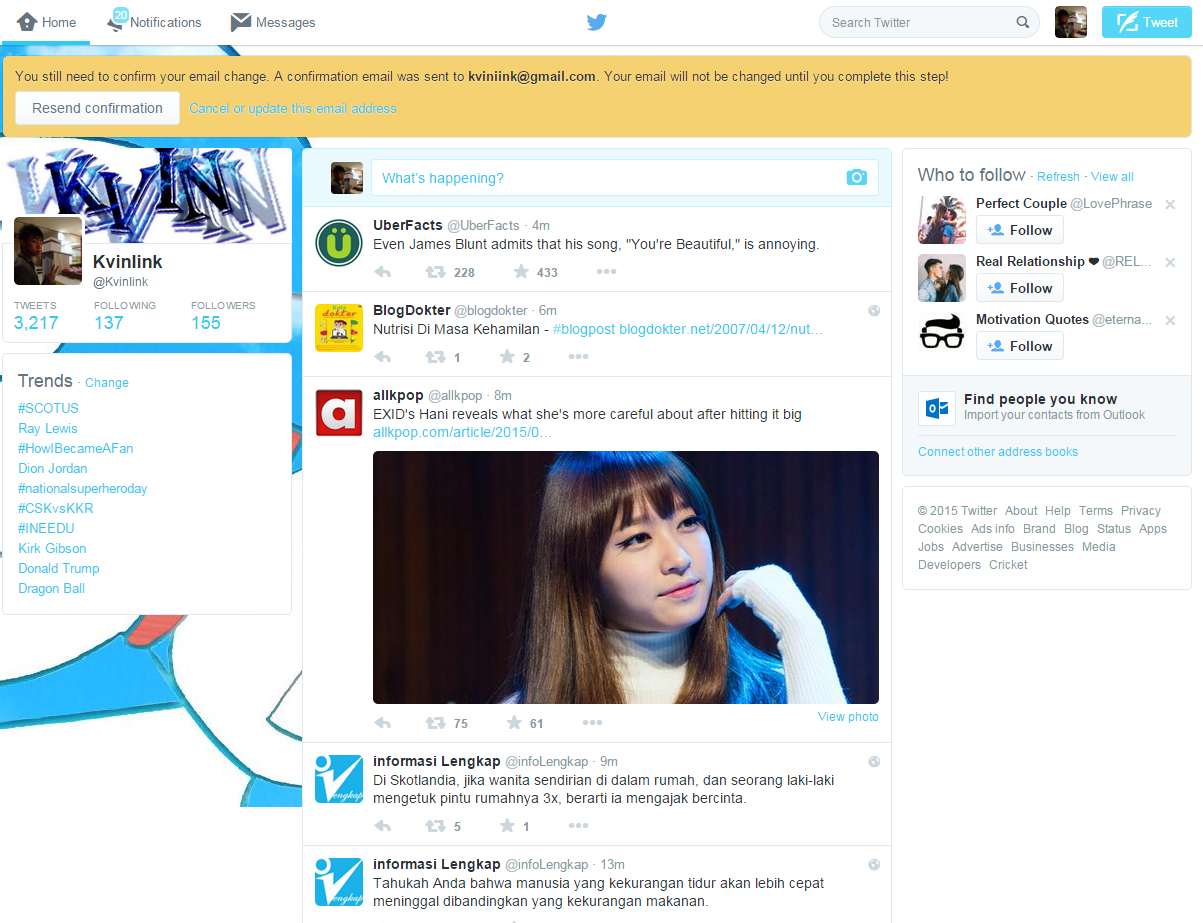
\includegraphics[width=1.00\textwidth]{C:/Skripsi/doc/DokumenSkripsi/Gambar/homePageTwitter.PNG}
	\caption{Home Page Twitter}
	\label{fig:homePageTwitter}
\end{figure}

\begin{figure}[htbp]
	\centering
		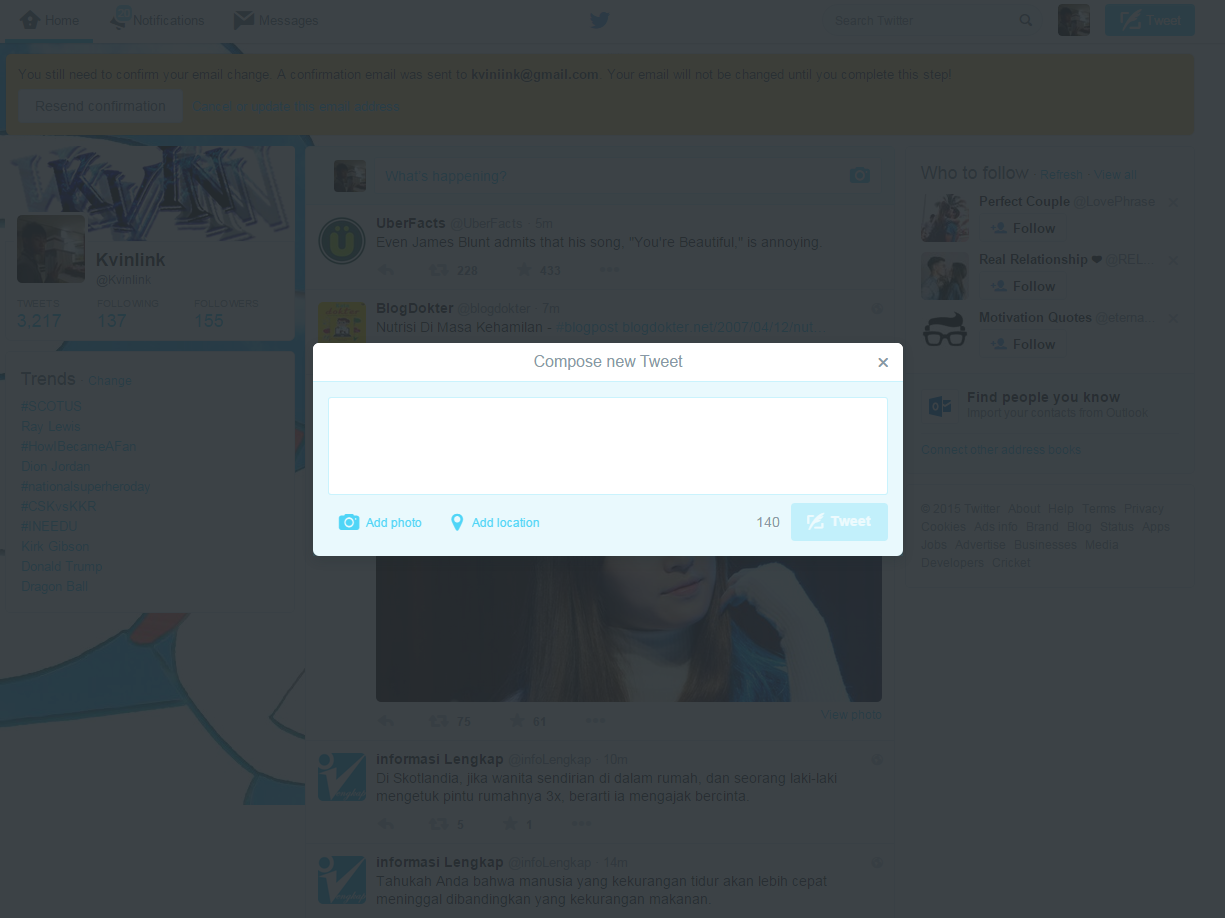
\includegraphics[width=1.00\textwidth]{C:/Skripsi/doc/DokumenSkripsi/Gambar/textboxTweetKlik.PNG}
	\caption{Tampilan untuk User Melakukan Tweet}
	\label{fig:textboxTweetKlik}
\end{figure}



\section{Pengujian}
\subsection{Pengujian Fungtional}
Pada subbab ini, akan dilakukan pengujian terhadap aplikasi pembuatan \textit{Twitter Bot} untuk mencari jalur transportasi publik.

Pertama kali aplikasi dijalankan, aplikasi akan melakukan otentifikasi untuk melakukan Twitter \textit{stream} yang dapat dilihat pada gambar ~\ref{fig:StartingProgram}.

\begin{figure}[htbp]
	\centering
		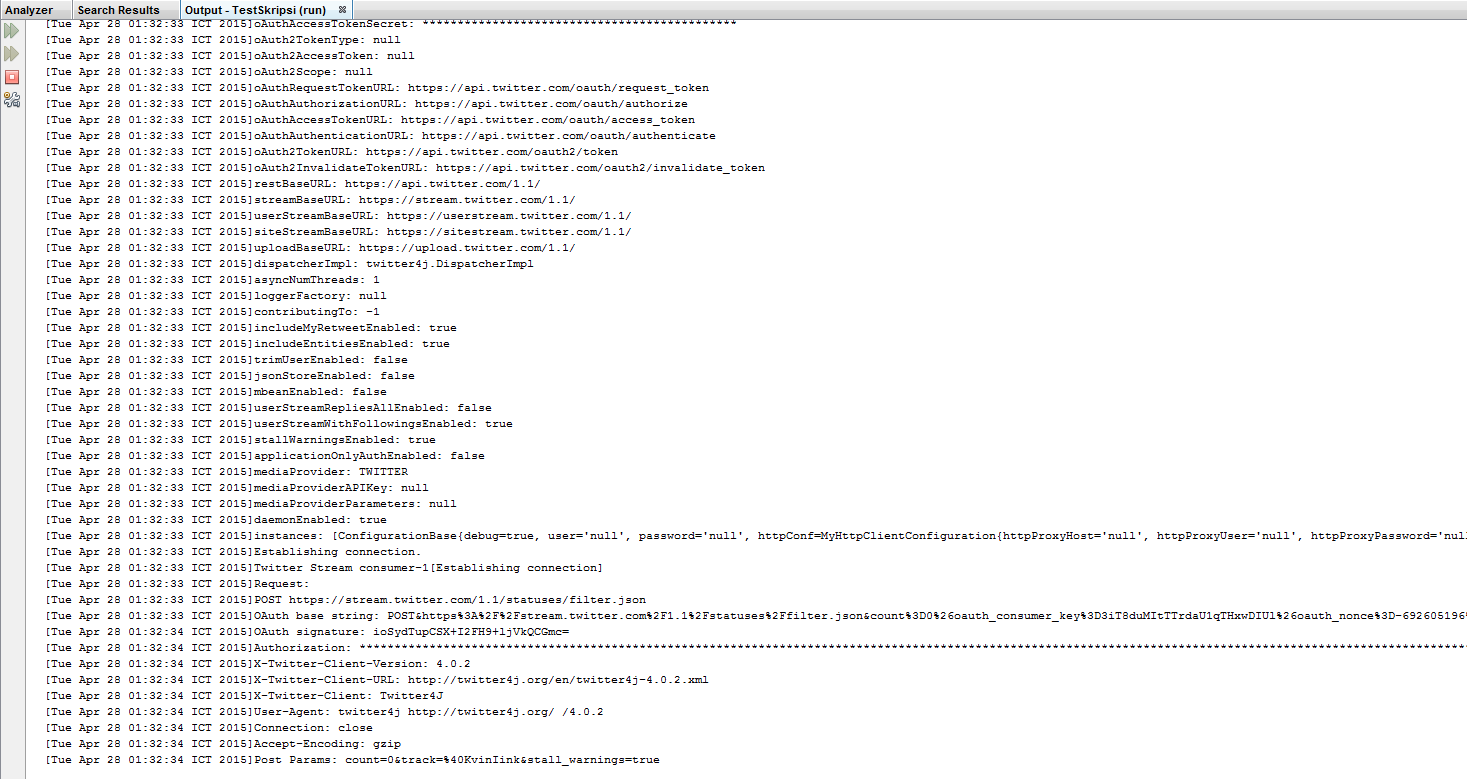
\includegraphics[width=1.00\textwidth]{C:/Skripsi/doc/DokumenSkripsi/Gambar/StartingProgram.PNG}
	\caption{Starting program}
	\label{fig:StartingProgram}
\end{figure}

??Textbox \textit{tweet}?? berfungsi untuk melakukan \textit{tweet}, disini user dapat menggunakannya untuk mencari jalur transportasi publik dengan cara melakukan \textit{mention} kepake @kiriupdate seperti yang ada di gambar ~\ref{fig:textboxTweet}.

\begin{figure}[htbp]
	\centering
		
\includegraphics[width=1.00\textwidth]{C:/Skripsi/doc/DokumenSkripsi/Gambar/textboxTweet.PNG}
	\caption{Compose new Tweet}
	\label{fig:textboxTweet}
\end{figure}

Setelah melakukan \textit{tweet}, dapat dilihat pada gambar ~\ref{fig:SuccessTweetToKiriUpdate}. Maka program akan menangkap tweet tersebut, dapat dilihat pada gambar ~\ref{fig:TweetDitangkap}. Setelah itu tweet tersebut akan diolah untuk dicari rute transportasi publik tersebut. ??Apakah program harus memberi tampilan tentang bagaimana data diolah step by stepnya, dimulai dari mencari koordinat lokasi awal dan tujuan, sampai dengan hasil pencariannya??. Ketika selesai aplikasi akan membalas \textit{tweet} jalur transportasi publik kepada \textit{user} seperti yang ada di gambar ~\ref{fig:HasilTweet}.

\begin{figure}[htbp]
	\centering
		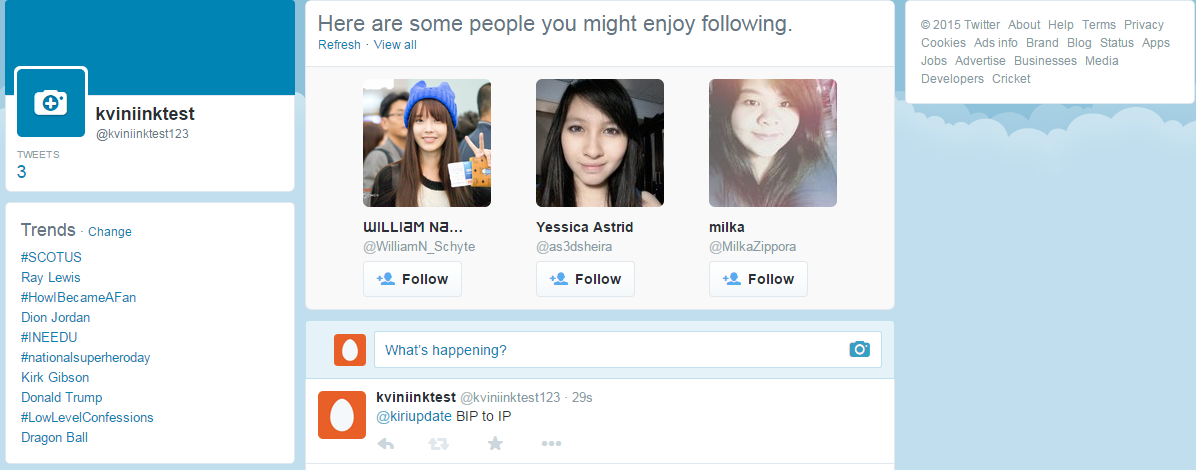
\includegraphics[width=1.00\textwidth]{C:/Skripsi/doc/DokumenSkripsi/Gambar/SuccessTweetToKiriUpdate.PNG}
	\caption{Tweet Kepada User @kiriupdate}
	\label{fig:SuccessTweetToKiriUpdate}
\end{figure}

\begin{figure}[htbp]
	\centering
		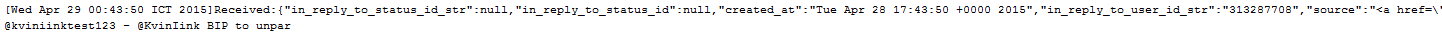
\includegraphics[width=1.00\textwidth]{C:/Skripsi/doc/DokumenSkripsi/Gambar/TweetDitangkap.PNG}
	\caption{Tweet Diterima oleh Aplikasi}
	\label{fig:TweetDitangkap}
\end{figure}

\begin{figure}[htbp]
	\centering
		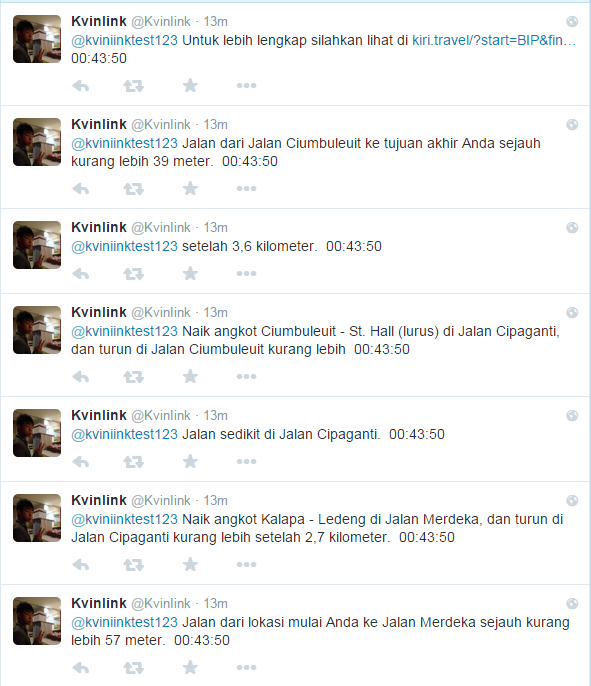
\includegraphics[width=1.00\textwidth]{C:/Skripsi/doc/DokumenSkripsi/Gambar/HasilTweet.PNG}
	\caption{Tweet Rute Jalur Transportasi Publik}
	\label{fig:HasilTweet}
\end{figure}

\subsection{Pengujian Eksperimental}
Pada subbab ini akan dilakukan pengujian \textit{Twitter Bot} untuk mencari jalur transportasi publik selama 12 jam.